\chapter{Алгоритм Mean Shift}
\section{Суть алгоритма}
Алгоритм кластеризации Mean Shift направлен на обнаружение сгустков плотности среди заданного
набора образцов. Он является центроидным, то есть работает посредством обновления положения центров
плотности. На каждой итерации алгоритма высчитывается среднее взвешенное значение плотности
образцов в заданной области с использованием особой функции, называемой ядром:
\[
    m(x) = \frac{\sum_{x_i \in N(x)} K(x_i - x)x_i}{\sum_{x_i \in N(x)} K(x_i - x)},
\]
где \( m(x) \)~-- среднее взвешенное значение плотности в заданной области, \( N(x) \)~--
соседние к \( x \) образцы, причем для них \( K(x) \ne 0 \), \( K(x_i - x) \)~-- ядро.

В ядре содержится единственный параметр, используемый в данном ал\-го\-рит\-ме:
\[
    K(x_i - x) = k\left( \frac{\|x_i - x\|^2}{h^2} \right).
\]
Параметр \( h \), называемый <<пропускной способностью>> (\emph{bandwidth}), в данном
ал\-го\-рит\-ме регулирует размер области, в которой ищутся соседние образцы и рассчитывается
среднее значение плотности. Функция \( k \) здесь -- профиль ядра.

Обычно в качестве ядра используют гауссианы:
\[
    K(x_i - x) = e^{-c\|x_i - x\|^2}.
\]

После расчета \( m(x) \) алгоритм заменяет положение центроидов \( x \) на рас\-счи\-тан\-ные
\( m(x) \), и переходит к следующей итерации.

В период пост-обработки центроиды фильтруются, отбрасываются дуб\-ли\-ка\-ты и близлежащие
центроиды, после чего формируется окончательный набор центроидов.

Сильные стороны алгоритма:
\begin{itemize}
    \item весь процесс кластеризации зависит только от одного параметра \( h \), имеющего реальный
        физический смысл;
    \item нет зависимости от размерности пространства и конкретной метрики расстояний;
    \item не предполагает конкретных форм кластеров.
\end{itemize}

Слабые стороны алгоритма:
\begin{itemize}
    \item выбор параметра \( h \) весьма нетривиален, зачастую требует адаптивной подстройки во
        время работы алгоритма; а неправильный выбор этого параметра может приводить к схопыванию
        кластеров или генерации дополнительных кластеров, в которых плотность образцов невелика;
    \item алгоритм является очень ресурсоемким: в общем он требует \( O(kN^2) \) операций, где
        \( N \)~-- число образцов, \( k \)~-- среднее количество итераций на один образец.
\end{itemize}

\begin{figure}[hp!]
    \center
    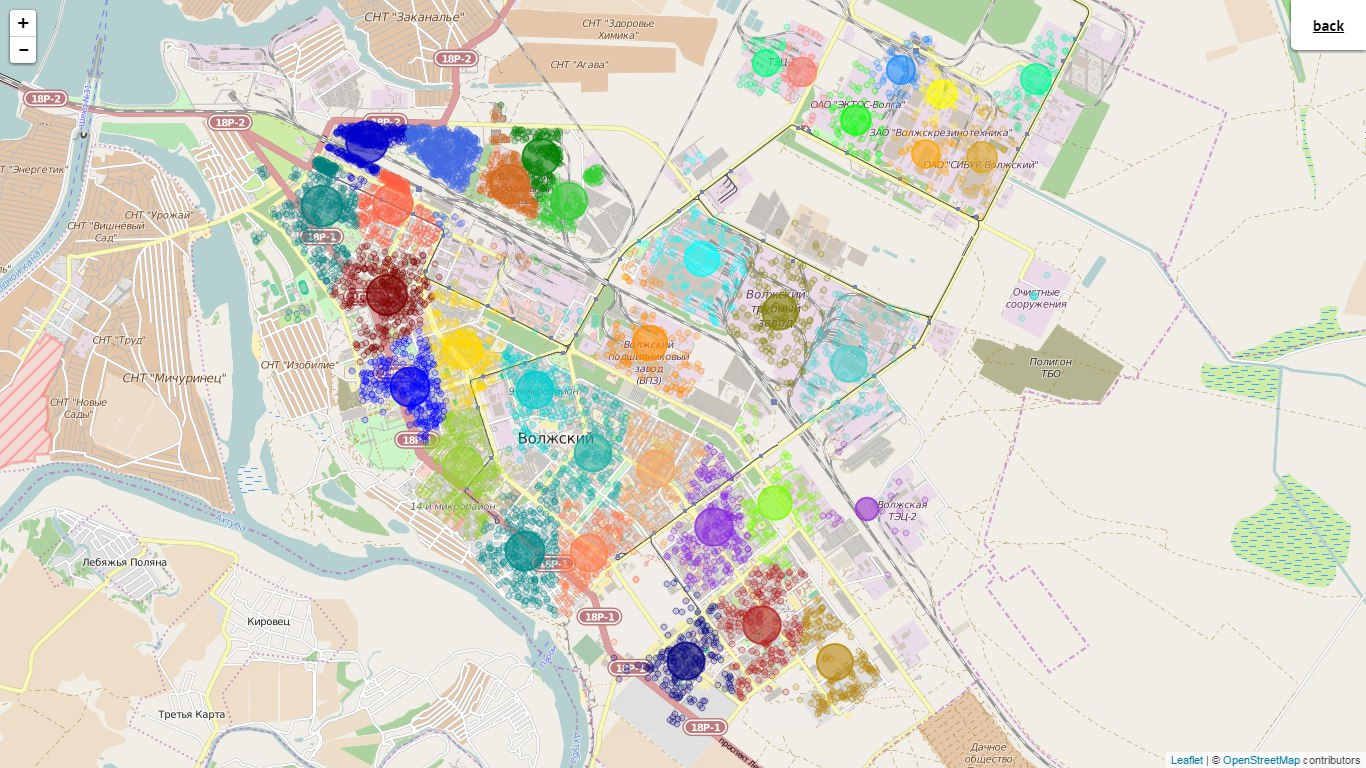
\includegraphics[width=1.0\textwidth]{km}\\
    \parbox{1.0\textwidth}{\centering\caption{Результаты кластеризации алгоритмом K-Means}}\\
    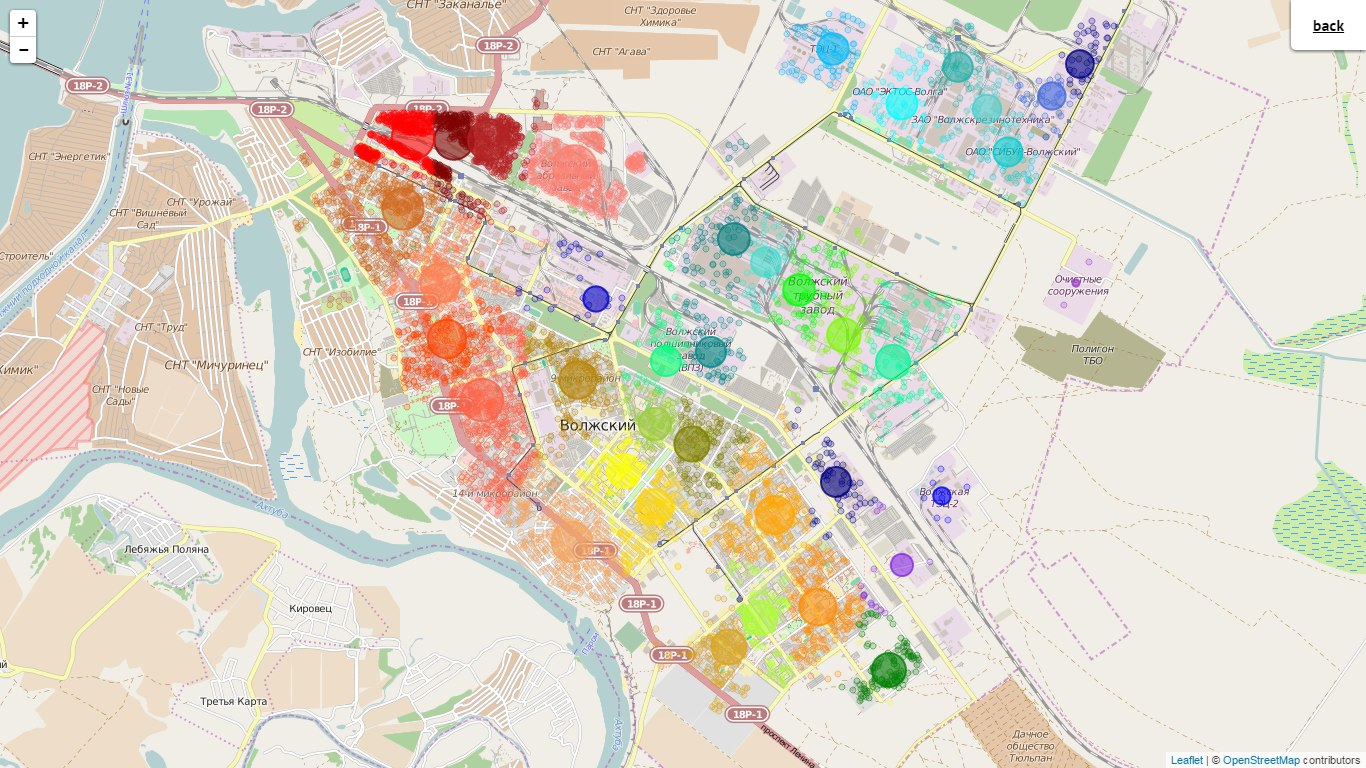
\includegraphics[width=1.0\textwidth]{mn}\\
    \parbox{1.0\textwidth}{\centering\caption{Результаты кластеризации алгоритмом Mean Shift}}
\end{figure}

\section{Реализация}
Алгоритм Mean Shift был реализован на языке программирования Python с использованием
библиотек numpy и sklearn. Также при написании ис\-поль\-зуют\-ся ранее написанные модули
ClusteringMachine и DataCollector. Реали\-за\-ция пред\-став\-ляет собой подключаемый модуль,
который можно запускать и как обыч\-ный Python-скрипт.

\lstinputlisting[language=Python, caption=Модуль DataCollector]{DataCollector.py}
\lstinputlisting[language=Python, caption=Модуль ClusteringMachine]{ClusteringMachine.py}
\lstinputlisting[language=Python, caption=Модуль MeanShift]{meanshift-simple.py}

\chapter{Построение маршрутов}
\section{Установка и настройка Project-OSRM}
Для нахождения расстояния между двумя точками с помощью построения маршрута между ними было решено
воспользоваться утилитой Project-OSRM (\url{http://project-osrm.org}).

Поскольку проект реализовывается на ОС Fedora, то следующие команды действительны для нее
(установку на других ОС можно посмотреть по ссылке:
\url{https://github.com/Project-OSRM/osrm-backend/wiki/Building-OSRM}).

Устанавливаем git, cmake и gcc для c++:
\begin{lstlisting}
$ sudo yum install git cmake gcc-c++
\end{lstlisting}

Далее устанавливаем все необходимые зависимости:
\begin{lstlisting}
$ sudo yum install libxml2-devel boost-devel boost-regex bzip2-devel \
  libzip-devel stxxl-devel protobuf-devel protobuf-lite protobuf-lite-devel \
  lua.x86_64 lua-devel.x86_64 luajit.x86_64 luajit-devel.x86_64 \
  luabind.x86_64 luabind-devel.x86_64 expat expat-devel tbb tbb-devel
\end{lstlisting}

Устанавливаем библиотеку для чтения и записи PBF файлов:
\begin{lstlisting}
$ git clone https://github.com/scrosby/OSM-binary.git
$ cd OSM-binary
$ cmake .
$ sudo make install
\end{lstlisting}

Устанавливаем Project-OSRM:
\begin{lstlisting}
$ git clone https://github.com/DennisOSRM/Project-OSRM.git
$ mkdir –p Project-OSRM/build
$ cd Project-OSRM/build
$ cmake ..
$ make
$ sudo make install
\end{lstlisting}

И, наконец, устанавливаем серверную часть Project-OSRM:
\begin{lstlisting}
$ git clone https://github.com/Project-OSRM/osrm-backend.git
$ cd osrm-backend
$ mkdir -p build
$ cd build
$ cmake ..
$ make
\end{lstlisting}

Теперь перейдем к настройке. Не выходя из директории \emph{build} делаем символическую ссылку
на скоростной профиль и директорию с библиотеками для скоростных профилей. Стандартным скоростным
профилем является профиль автомобиля:
\begin{lstlisting}
$ ln -s ../profiles/car.lua profile.lua
$ ln -s ../profiles/lib/
\end{lstlisting}

Скачиваем какую-либо OpenStreetMap-карту, в моем случае -- карту Вол\-го\-град\-ской области, и
распаковываем ее:
\begin{lstlisting}
$ ./osrm-extract map.osm
\end{lstlisting}

На выходе получаем файл \emph{map.osrm}. Далее, выполняем обработку данных с карты:
\begin{lstlisting}
$ ./osrm-prepare map.osrm
\end{lstlisting}
На выходе получаем набор из 9 файлов, каждый из которых содержит какую-либо определенную часть
карты OpenStreetMap.

Теперь всё готово для запуска сервера с Project-OSRM. Для этого ис\-поль\-зуем команду
\begin{lstlisting}
$ ./osrm-routed map.osrm
\end{lstlisting}

\section{Реализация метрики}
Реализуемая метрика была названа \emph{route}. Модуль содержит класс \emph{route},
в котором есть три функции: \emph{start}, \emph{stop} и \emph{route\_distance}.

Первая функция запускает процесс \emph{osrm-routed} с нужным файлом карты.

Вторая функция останавливает запущенную OSRM машину.

Третья функция возвращает дистанцию между двумя точками, пе\-ре\-дан\-ных ей в качестве параметров.

\lstinputlisting[language=Python, caption=Модуль route]{route.py}

\chapter{Внедрение метрики}
\section{Внедрение метрики в алгоритм K-Means}
В модуль k-means внедрение метрики довольно просто. Импортируем мо\-дуль:
\lstinputlisting[language=Python,firstline=8,lastline=8]{kmeans.py}

Добавляем поле \emph{route\_} классу, который отвечает за расчет расстояний.
Прописываем этот расчет:
\lstinputlisting[language=Python,firstline=115,lastline=139]{kmeans.py}

Далее, в функции, отвечающей за кластеризацию, прописываем запуск и остановку OSRM машины:
\lstinputlisting[language=Python,firstline=180,lastline=181]{kmeans.py}
\lstinputlisting[language=Python,firstline=229,lastline=230]{kmeans.py}

В итоге просто указываем необходимую метрику:
\lstinputlisting[language=Python,firstline=337,lastline=360]{kmeans.py}

\section{Внедрение метрики в алгоритм Mean Shift}
С внедрением метрики в модуль с алгоритмом Mean Shift всё гораздо сложнее.

Во-первых, метрика никак не была задана изначально. Во-вторых, сам алгоритм не находится
<<на виду>>, а реализован внутри подключенной библиотеки.

Решением является необходимое изменение библиотеки.

Для начала добавим запуск и остановку OSRM машины в написанный модуль:
\lstinputlisting[language=Python,firstline=7,lastline=9]{meanshift.py}
\ldots
\lstinputlisting[language=Python,firstline=29,lastline=33]{meanshift.py}
\ldots
\lstinputlisting[language=Python,firstline=44,lastline=51]{meanshift.py}
\ldots

Далее, скачиваем библиотеку scikit-learn и начинаем добавлять реализованную метрику:
\begin{lstlisting}
$ git clone https://github.com/scikit-learn/scikit-learn.git
\end{lstlisting}

Внутри находим директорию \emph{sklearn}, в ней и содержится Python-библиотека.
Кладем в корень директории модуль метрики.

Алгоритм Mean Shift находится в файле \emph{cluster/mean\_shift\_.py}.
Добавляем выбор метрики: везде параметром прописываем \emph{metric = 'route'}.

Далее, нужно написать саму метрику, чтобы алгоритм мог ее выбрать. В \emph{metrics/pairwise.py}
добавляем новую метрику и прописываем в списках доступных метрик новую.

Для того, чтобы алгоритм поиска соседей тоже мог пользоваться нашей метрикой, прописываем нашу
метрику в файл \emph{neighbors/dist\_metric.pyx}. Для сохранения сделанных изменений в этом файле
необходимо скомпилировать c-библиотеку:
\begin{lstlisting}
$ cd neighbors
$ cython dist_metric.pyx
\end{lstlisting}

Добавляем нашу прописанную метрику в список доступных метрик в файле с алгоритмом поиска соседей
\emph{neighbors/ball\_tree}.

При первом запуске начальные центры кластеров становятся в точку с координатами \texttt{(0, 0)}.
Чтобы этого избежать, в файле с алгоритмом Mean Shift (\emph{cluster/mean\_shift\_.py}) находим
строчку:
\begin{lstlisting}[language=Python]
binned_point = np.round(point / bin_size)
\end{lstlisting}

В этом месте для упрощения расчетов координаты делятся на размер рассматриваемой области
и округляются. В нашем случае такое поведение не подходит -- размер области на 1-2 порядка
превышает координаты. Поэтому выберем определенное количество цифр после запятой, которые будут
оставаться после округления:
\begin{lstlisting}[language=Python]
binned_point = np.round(point / bin_size, decimals = 5)
\end{lstlisting}

Теперь всё готово для тестов -- собираем и устанавливаем измененную библиотеку:
\begin{lstlisting}
$ cd scikit-learn
$ python setup.sh build
$ sudo python setup.sh install
\end{lstlisting}

Теперь вместо библиотеки \emph{scikit-learn} у нас установлена ее измененная версия.
Таким образом, алгоритм Mean Shift также поддерживает новую метрику.

На один запрос расчета дистанции между двумя точками требуется примерно 10~мсек.
На то, чтобы рассчитать только расстояния между всеми точками тестовой выборки (6000 точек)
необходимо потратить:
\[
    t = \frac{6000!}{2 * 5998!} \cdot 10 = 179970000\textrm{ мсек} \approx 50\textrm{ ч}.
\]
